\section*{Errata}
\setlength{\parindent}{0pt}

On page~44, in the first line of Equation~3.48, there was a missing $\delta$ before $\qpdensity(\time)$.

On page~46, the sentence immediately following Equation~3.54 should read
\begin{quote}
Even for large perturbations where $\qprecombinationeff \qprelaxationtime \, \delta\qpdensity(0) \gg 1$, after a time of order $\qprelaxationtime$ the system will have recovered to an excess density $\delta\qpdensity \sim (\qprecombinationeff \qprelaxationtime)^{-1} = 2 \ssqpdensity + \qpsingledecay / \qprecombinationeff$.
\end{quote}

Equations~3.79 and 3.80 contained errors.
A sentence immediately following these equations and Figure~3.12 (reproduced below) have been updated accordingly.
Equation~3.79:
\begin{equation*}
\normresponse_{\reconductivity}(\temperature)
  =
  \left( \frac{8 \gap_\zerotemp}{\pi^3 \kb \temperature} \right)^{1/2}
  \sinh \left( \frac{\planck \freadout}{2 \kb \temperature} \right)
  K_0 \left( \frac{\planck \freadout}{2 \kb \temperature} \right).
\end{equation*}
Equation~3.80:
\begin{equation*}
\normresponse_{\imconductivity}(\temperature)
  =
  - \left[
  1 + \left( \frac{2 \gap_\zerotemp}{\pi \kb \temperature} \right)^{1/2}
  \exp \left( -\frac{\planck \freadout}{2 \kb \temperature} \right)
  I_0 \left( \frac{\planck \freadout}{2 \kb \temperature} \right)
  \right].
\end{equation*}
\begin{figure}[!h]
\centering
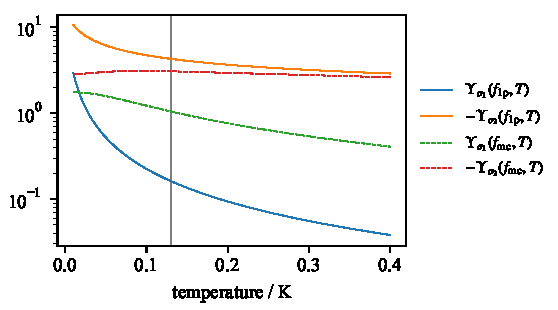
\includegraphics[width=0.8\textwidth]{theory/normresponse_conductivity_thermal.pdf}
\end{figure}
\clearpage

Equations~3.91 through~3.96 contained some typos and inconsistent notation, and should read as given below. Equation~3.91:
\begin{equation*}
\ssloss_\quasiparticle
  =
  \frac{\kifraction}{\reactance_\surface(0)}
  \frac{\surfimpexp \reactance_\surface(0)}{\imconductivity(0)}
  \ssreconductivity
  =
  \frac{\kifraction \surfimpexp}{\imconductivity(0)}
  \braket*{\responseqpoccupancy_{\reconductivity}}{\ssqpoccupancy}.
\end{equation*}
Equation~3.92:
\begin{equation*}
\ssshift
  =
  \frac{\kifraction}{2 \reactance_\surface(0)}
  \left( -\frac{\surfimpexp \reactance_\surface(0)}{\imconductivity(0)} \right)
  \left[ \ssimconductivity - \imconductivity(0) \right]
  =
  -\frac{\kifraction \surfimpexp}{2 \imconductivity(0)}
  \braket*{\responseqpoccupancy_{\imconductivity}}{\ssqpoccupancy}.
\end{equation*}
Equation~3.93:
\begin{align*}
\begin{split}
\delta\loss_\quasiparticle(\time)
  =
  \pdv{\loss_\quasiparticle}{\resistance_\surface}
  \pdv{\resistance_\surface}{\reconductivity}
  \delta\reconductivity(\time)
  &=
  \frac{\kifraction \surfimpexp}{\imconductivity(0)}
  \braket*{\responseqpoccupancy_{\reconductivity}}{\delta\qpoccupancy(\time)} \\
  &=
  \frac{\kifraction \surfimpexp}{\imconductivity(0)}
  \frac
  {\braket*{\responseqpoccupancy_{\reconductivity}}{\ssqpoccupancy}}
  {\braket*{\responseqpoccupancy_{\qpnumber}}{\ssqpoccupancy}}
  \braket*{\responseqpoccupancy_{\qpnumber}}{\delta\qpoccupancy(\time)} \\
  &=
  \frac{\kifraction \surfimpexp \ssnormresponse_{\reconductivity}}{2 \ssdos \gap_\zerotemp \volume} \delta\qpnumber(\time),
\end{split}
\end{align*}
where $\ssnormresponse_{\reconductivity} = \normresponse_{\reconductivity}[\ssqpoccupancy]$.
Equation~3.94:
\begin{align*}
\begin{split}
\delta\detuning(\time)
  =
  \pdv{\detuning}{\reactance_\surface}
  \pdv{\reactance_\surface}{\imconductivity}
  \delta\imconductivity(\time)
  &=
  -\frac{\kifraction \surfimpexp}{2 \imconductivity(0)}
  \braket*{\responseqpoccupancy_{\imconductivity}}{\delta\qpoccupancy(\time)} \\
  &=
  -\frac{\kifraction \surfimpexp}{2 \imconductivity(0)}
  \frac
  {\braket*{\responseqpoccupancy_{\imconductivity}}{\ssqpoccupancy}}
  {\braket*{\responseqpoccupancy_{\qpnumber}}{\ssqpoccupancy}}
  \braket*{\responseqpoccupancy_{\qpnumber}}{\delta\qpoccupancy(\time)} \\
  &=
  -\frac{\kifraction \surfimpexp \ssnormresponse_{\imconductivity}}{4 \ssdos \gap_\zerotemp \volume} \delta\qpnumber(\time),
\end{split}
\end{align*}
where
$\ssnormresponse_{\imconductivity} = \normresponse_{\imconductivity}[\ssqpoccupancy]$
and 
$\delta\imconductivity = \imconductivity - \ssimconductivity$.
Equation~3.95:
\begin{equation*}
\delta\loss_\quasiparticle(\faudio)
  =
  \frac{\kifraction \surfimpexp \ssnormresponse_{\reconductivity}}{2 \ssdos \gap_\zerotemp \volume}
  \frac{\qprelaxationtime}{1 + 2 \pi \I \faudio \qprelaxationtime}
  \delta\Rate_\generation(\faudio).
\end{equation*}
Equation~3.96:
\begin{equation*}
\delta\detuning(\faudio)
  =
  -\frac{\kifraction \surfimpexp \ssnormresponse_{\imconductivity}}{4 \ssdos \gap_\zerotemp \volume}
  \frac{\qprelaxationtime}{1 + 2 \pi \I \faudio \qprelaxationtime}
  \delta\Rate_\generation(\faudio).
\end{equation*}
